\documentclass[12pt]{article}
\usepackage{amsmath,amsfonts, epsfig}
\usepackage{booktabs} % for better table formatting
\usepackage{array}
\usepackage{multirow}
\usepackage{graphicx}
\usepackage{fancyhdr}
\usepackage{bm}
\pagestyle{fancy}
\lfoot{\texttt{ematm0067.github.io}}
\lhead{Introduction to AI - 03.1\_perceptron - Conor}
\rhead{\thepage}
\cfoot{}

\usepackage{tikz}
\usetikzlibrary{positioning}

\usetikzlibrary{shapes.misc}


\usepackage{ifthen,calc}
\newboolean{nopics}
\setboolean{nopics}{false}


\begin{document}

\section*{A linear classifier.} 

In the last section we looked at linear classifiers; this was a
reinterpretation of regression as a classifier, effectively using a
line, in two-dimensions, or a hyper-plane in more dimensions, to
divide the space into two halves, one hopefully mostly ducks, the
other mostly rabbits, or whatever it is you are trying to
classify. The big problem with this is that it assumes the division is
created by a straight line or flat plane or whatever; the linear in
linear classifier is a big restriction on the manner you can seperate the data, it can deal with this:
\begin{center}
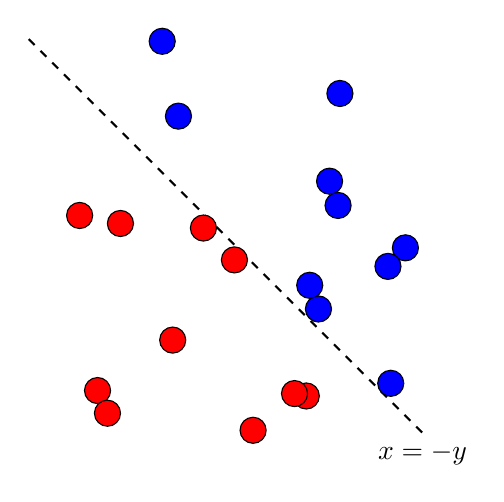
\begin{tikzpicture}[x=0.5cm, y=0.5cm]
% Set the size of the figure
\draw[white] (-5,-5) rectangle (5,5); 

% Draw the line x = -y
\draw[thick, dashed] (-5,5) -- (5,-5) node[below] {\(x = -y\)};
 \node[draw, circle, fill=blue] at (2.903034362374342,3.6206140956417148) {};
\node[draw, circle, fill=blue] at (-1.1988721079670475,3.0444741580278993) {};
\node[draw, circle, fill=blue] at (4.5659497841882395,-0.3003318387195364) {};
\node[draw, circle, fill=blue] at (2.357629434628535,-1.8536739644484412) {};
\node[draw, circle, fill=blue] at (-1.611019883900732,4.946323932639682) {};
\node[draw, circle, fill=blue] at (4.193907059591499,-3.741317007274522) {};
\node[draw, circle, fill=blue] at (2.8559910586751167,0.7766901004173965) {};
\node[draw, circle, fill=blue] at (2.6401256324946125,1.392419554199149) {};
\node[draw, circle, fill=blue] at (2.136250524167779,-1.2519337352619955) {};
\node[draw, circle, fill=blue] at (4.122742742830933,-0.7715993829424752) {};
\node[draw, circle, fill=red] at (2.048733156460959,-4.06293497368835) {};
\node[draw, circle, fill=red] at (-2.6716005375553467,0.31811554721441304) {};
\node[draw, circle, fill=red] at (1.750115261826589,-4.002160389726505) {};
\node[draw, circle, fill=red] at (-3.7079565474866993,0.5216001531036785) {};
\node[draw, circle, fill=red] at (-3.2533866989281277,-3.925347364746198) {};
\node[draw, circle, fill=red] at (-3.0015205876441176,-4.501361878836062) {};
\node[draw, circle, fill=red] at (0.22346837368476358,-0.6067570329114318) {};
\node[draw, circle, fill=red] at (0.6975960506611205,-4.934609123738221) {};
\node[draw, circle, fill=red] at (-1.344066710177355,-2.6437221154587656) {};
\node[draw, circle, fill=red] at (-0.5643289400416887,0.20253932887644766) {};
\end{tikzpicture}
\end{center}
but it can't deal with this:
\begin{center}
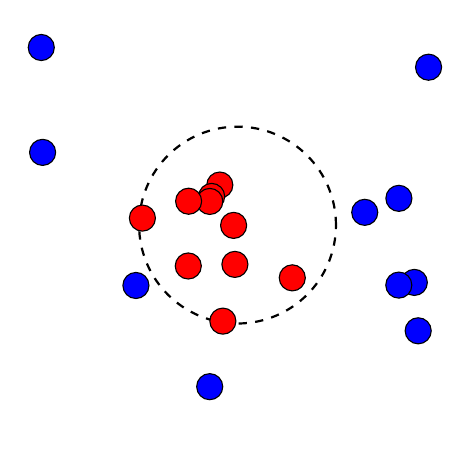
\begin{tikzpicture}[x=0.5cm, y=0.5cm]

% Set the size of the figure
\draw[white] (-5,-5) rectangle (5,5); 

% Draw the line x = -y
\draw[thick,dashed] (0,0) circle [radius=2.5];
\node[draw, circle, fill=blue] at (4.490346586522341,-1.4562378730751324) {};
\node[draw, circle, fill=blue] at (4.588503013754599,-2.685479987653314) {};
\node[draw, circle, fill=blue] at (4.0985940838479955,0.6791623208691346) {};
\node[draw, circle, fill=blue] at (3.2310962258872404,0.3236015658341538) {};
\node[draw, circle, fill=blue] at (-4.951072578691123,1.846660618411522) {};
\node[draw, circle, fill=blue] at (-0.7067234028777847,-4.10444514907131) {};
\node[draw, circle, fill=blue] at (-2.580917460236928,-1.534016306483481) {};
\node[draw, circle, fill=blue] at (4.852584733382379,4.009744362360637) {};
\node[draw, circle, fill=blue] at (-4.985104113776853,4.510524821482017) {};
\node[draw, circle, fill=blue] at (4.096236058228337,-1.524542756843469) {};
\node[draw, circle, fill=red] at (-0.37251466326944893,-2.4396858821202594) {};
\node[draw, circle, fill=red] at (-2.4164802515905137,0.1770845040212956) {};
\node[draw, circle, fill=red] at (-0.09942463793439771,-0.007984259123821502) {};
\node[draw, circle, fill=red] at (-0.45019655042723095,1.0165475244338564) {};
\node[draw, circle, fill=red] at (-0.06671294409036133,-0.9985234990220668) {};
\node[draw, circle, fill=red] at (-1.2508913539186084,-1.038936199084739) {};
\node[draw, circle, fill=red] at (-0.6574936711542767,0.7279760311071373) {};
\node[draw, circle, fill=red] at (-0.7048668988542222,0.6006558362141954) {};
\node[draw, circle, fill=red] at (-1.2422205380080085,0.6059517202449065) {};
\node[draw, circle, fill=red] at (1.3904669431542613,-1.3404347066072941) {};
\end{tikzpicture}
\end{center}
We will have a look, in a broad way, at the solution to this
problem. In short we will use a larger class of seperating lines
defined by a neural network. However, this is a sort of `modern' way
of look the problem, it was actually discovered using a more
roundabout analogy with neuroscience and so we will take a short
segway though that way of framing neural networks, the `neural'
approach as it were. This will mean rephrasing the linear classifier as a \textsl{perceptron}.

\section*{Modelling the brain}

\subsection*{The McCulloch-Pitts neuron}


The McCulloch Pitts neuron model, or Threshold Logic Unit, was
introduced in 1943 by Warren McCulloch and Walter
Pitts\footnote{Walter Pitts was an interesting and odd man, a genius
in the old-fashioned self-destructive and brilliant sense.} as a
computational model of a neuronal network
\cite{McCullochPitts1943}. Their thinking was that neurons are joined
to each other with connections of variable strength; in the soma the
inputs from other neurons are added up and they determine the activity
of the neuron in a non-linear way; they also knew that neurons tend to
ignore input up to some threshold value before responding
strongly. These properties they tried to include in their model
neurons.

Artificial neurons, of the sort used in artificial intelligence, are
described by a single dynamical variable, $x_i$ say for a neuron
labelled $i$; the value of $x_i$ is determined by the weighted input
from the other neurons:
\begin{equation}
x_i=\phi\left(\sum_j w_{ij} x_j-\theta_i\right)
\end{equation}
$\phi$ is an activation function, $\theta$ is a threshold and the
$w_{ij}$ are the connection strengths weighting the inputs from the
other neurons. The McCulloch Pitts neuron was the first example of an
artificial neuron and had a step function for $\phi$:
\begin{equation}
x_i=\left\{\begin{array}{ll}1&\sum_j w_{ij} x_j>\theta_i\\-1&\mbox{otherwise}\end{array}\right.
\end{equation}
This step function is often called the \textsl{Heaviside} function.

Thus, the neuron has two states, it is in the on state, $x_i=1$ if the
weighted input exceeds a threshold $\theta_i$ and an off state,
$x_i=-1$ if it doesn't; the picture you might have of how this
corresponds to the brain is that \lq{}on\rq{} corresponds to rapid
spiking and \lq{}off\rq{} to spiking at a much lower rate.  For
McCulloch and Pitts this was the simplest way they could model the
properties that neurons had been observed to have of being silent
below some threshold. Now neurons above their threshold do increase
their activity as the input increases and this is one of the many ways
that the McCulloch-Pitts neuron was a simplification. It was useful at
the time because McCulloch and Pitts wanted to model these neurons
using simple electrical circuits at a time when computing was in its
infancy. They hoped, in fact, that these threshold units, as they
called them, would form the basis of computer architectures, as we
know this didn't happen, instead computers were built out of small
logical units. These days the simple on-off-ness of these units is
inconvenient and different activation functions are used, such as ReLU, we will return to this.


The $w_{ij}$, the connection strengths. For those of you who are
interested these are like the synapse strengths, a positive $w_{ij}$
is an excitatory synapse and negative, an inhibitory; a given neurons
have both negative and positive out-going synapses, that is there is
no restriction that says $w_{ij}$ always has the same sign for a given
$j$, this is different from real neurons where all the outgoing
synapses from a given neuron are either excitatory or inhibitory.

While it should be clear that this network has some of the properties,
very abstracted, of a neuronal network, it might not be so clear what
can be done with the neurons. When they were working, at the dawn of
the age of electronic computers, McCulloch and Pitts believed that
their neurons might form the natural unit in computer circuits. In
other words, they thought they might perform the role actually played
by logical circuits. In fact, it is still not clear if the artificial
neuron is or isn't the natural unit of computation since they are a
component in, for example, deep learning networks. In fact, there are
two major applications of McCulloch-Pitts neurons: the perceptron and
the Hopfield network. These two applications add a rule for changing
the connection strength to the original McCulloch-Pitts neuron.


\subsection*{Perceptrons}

The perceptron is a machine that does supervised learning, that is, it
makes guesses, is told whether or not its guess is correct, and then
makes another guess. They were first discovered in 1957 by Frank
Rosenblatt \cite{Rosenblatt1958} and introduced to the world with great fanfare, it was
claimed that they would solve problems from object recognition to
consciousness: if you consider the perceptron as the forbearer of the
deep learning network, then perhaps we don't know if these claims will
be fulfilled, but we do know that the original perceptron proved quite
limited in artificial intelligence. It does, however, appear to
describe some neuronal processes, if we ignore the implementation
details.

Anyway, a perceptron is made of two layers of neurons, an input layer
and an output layer of McCulloch-Pitts neurons. For simplicity let's
assume the output layer
has a single neuron.
\begin{center}
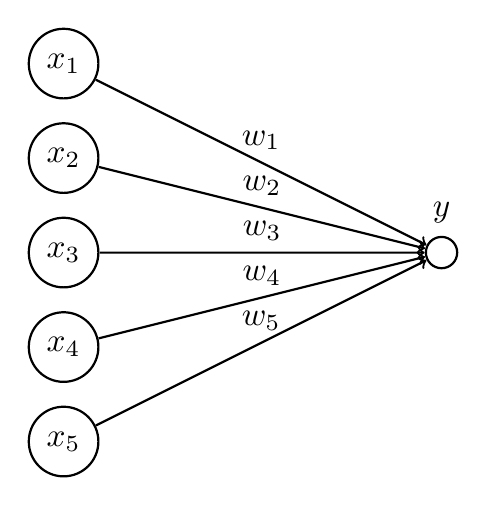
\begin{tikzpicture}[thick, scale=1.2, every node/.style={scale=1.2}]

% Input neurons
\foreach \i in {1,...,5} {
    \node[circle, draw, fill=white] (x\i) at (0,-\i) {$x_{\i}$};
}

% Output neuron
\node[circle, draw, fill=white] (output) at (4,-3) {};

% Connections with weights
\foreach \i in {1,...,5} {
    \draw[->] (x\i) -- (output) node[midway, above] {$w_{\i}$};
}

% Labels
\node[above] at (output.north) {$y$};

\end{tikzpicture}
\end{center}
Now, if the input is given by
$\textbf{x}=(x_1,x_2,\ldots,x_n)$ the output, $y$, is
\begin{equation}
y=\phi(r)
\end{equation}
where
\begin{equation}
r=\sum_j w_j x_j-\theta
\end{equation}
and $\phi$ here is the simple Heaviside-like activation function. Now for a given input, if the actual value of the
output should be $d$ the error is $d-y$. The perceptron learning rule
is to change the $w_j$ weight by an amount proportional to the error
and how much $x_j$ was \lq{}to blame\rq{} for the error:
\begin{equation}
\delta w_j=\eta (d-y) x_j
\end{equation}
and
\begin{equation}
\delta \theta =  \eta (d-y)
\end{equation}
where $\eta$ is some small learning rate and
\begin{eqnarray}
w_j&\rightarrow& w_j+\delta w_j\cr
\theta&\rightarrow& \theta+\delta\theta
\end{eqnarray}
You can see how this might work, if $x_j$ was positive and $y$ was too
big, this would make $w_j$ smaller so in future $y$ would be smaller
when it had the same input. 

In fact, the perceptron can only solve problems with a linear
classifier: if we think of the $x_i$'s as parametrizing an
$n$-dimensional space then $\sum_iw_ix_i=\theta$ is a hyperplane in
that space, so a pattern $\textbf{x}$ is classified one way or the
other according to which side of that hyperplane it lies, see for example Fig.~\ref{fig:linear_classifier}. Thus, the
perceptron works only if there is a hyperplane dividing the data into
two, with one class of data on one side and one on the other. In fact,
if the data is linearly separable the perceptron is guaranteed to
converge to a solution which manages this separation. Now, as
illustrated in Fig.~\ref{fig:random_points}, there will not be a unique
hyper-plane separating the two classes and the perceptron won't,
typically, find what you might regard as the \lq{}best\rq{}
hyperplane, where by best you might mean the line that is, in some
sense, as far from the individual data points as possible; finding
that best hyperplane is the idea behind the support vector machine.


\begin{figure}
  \ifthenelse{\boolean{nopics}}
               {{\textsl{In the figure the line $1.1x_1+x_2=0.25$ divides the plane into two halves, there are ten randomly placed red points one side of the line, ten randomly placed blue points the other. The area above the line is shaded light grey.}}}
                            {
\begin{center}  
  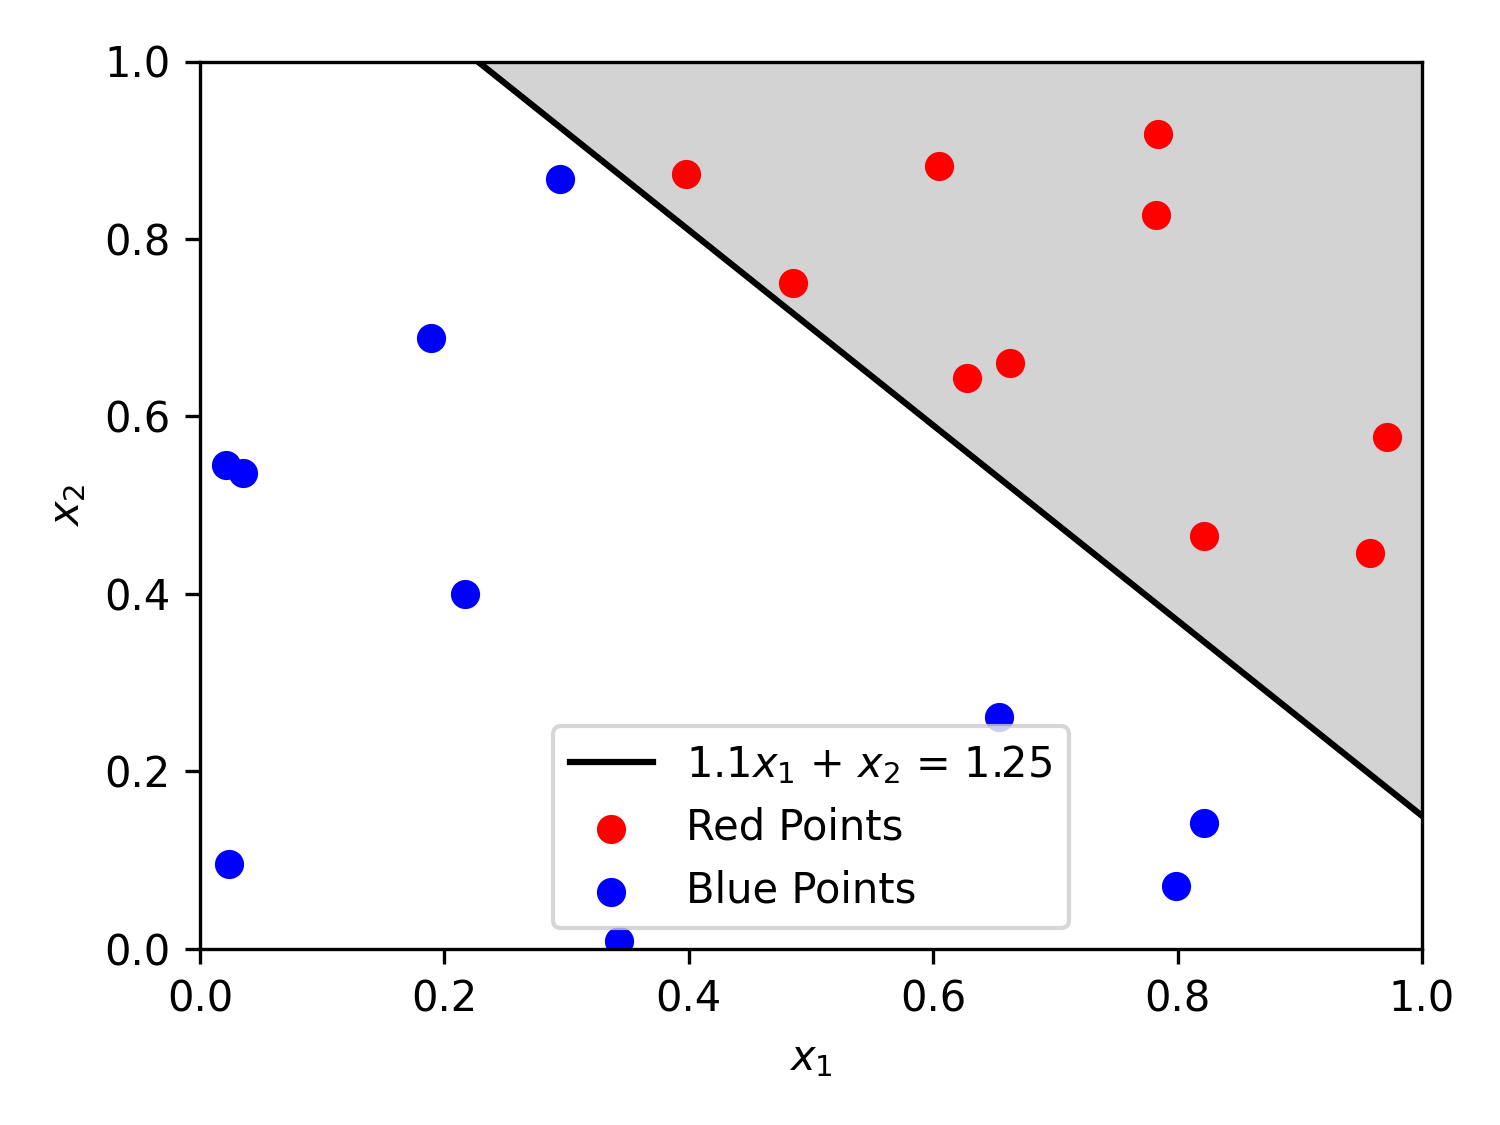
\includegraphics{linear_classifier.png}
\end{center}
}
\caption{Here the shaded region corresponds to $1.1x_1+x_2>0.25$, so
  if $w_1=1.1$ and $w_2=1$ with $\theta=0.25$ then the corresponding
  perceptron neuron will be one for all the circle points and -1 for
  all the square points.\label{fig:linear_classifier}}
\end{figure}


\begin{figure}
  \ifthenelse{\boolean{nopics}}
               {{\textsl{In the figure the line $1.1x_1+x_2=0.25$ divides the plane into two halves, there are ten randomly placed red points one side of the line, ten randomly placed blue points the other. There are three additional dotted lines close to the main $1.1x_1+x_2=0.24$, these lines also separate the points in a red group and a blue group.}}}
                            {
\begin{center}  
  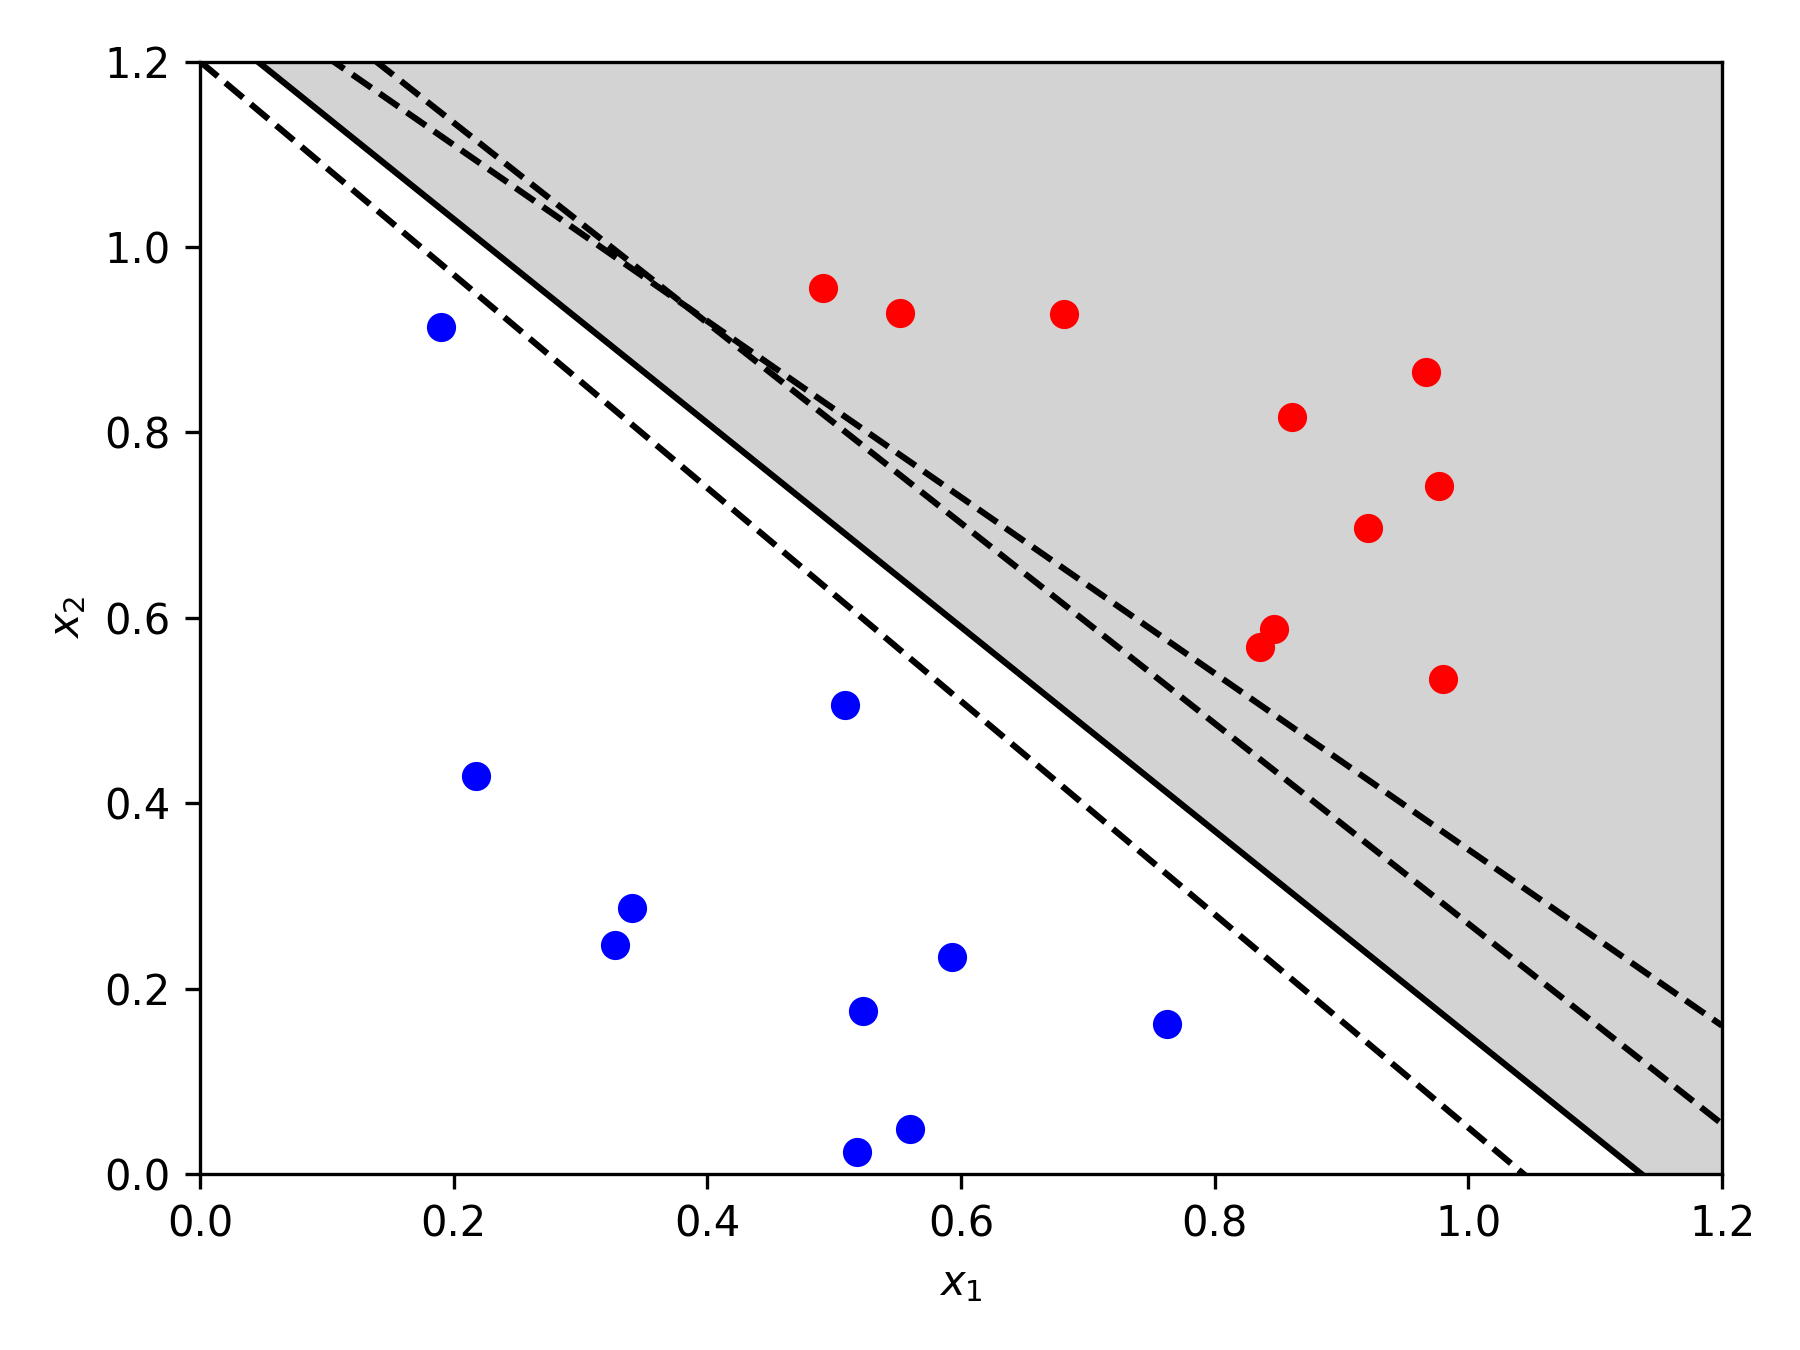
\includegraphics{random_points.png}
\end{center}
}\caption{All of these lines separate the points into two classes\label{fig:random_points}}
\end{figure}

The perceptron learning rule can be motivated by thinking about error
minimization. Consider an error function
\begin{equation}
E=\langle(d^a-y^a)^2\rangle_a
\end{equation}
If $a$ labels lots of input, $\textbf{x}^a$, desired output $d^a$
pairs, with $y^a$ the actual output; the angle brackets are an average
over these pairs. Now consider the gradient of $E$ with $w_{i}$:
\begin{equation}
\frac{\partial E}{\partial w_{i}}=-2\left\langle (d^a-y_a) \frac{\partial y^a}{\partial w_{i}}\right\rangle
\end{equation}
Now if we ignore for the moment the fact that the activation function for the McCulloch-Pitt neuron isn't differentiable and write
\begin{equation}
y^=\phi(r)
\end{equation}
with 
\begin{equation}
r=\sum_{i}w_i x_i-\theta
\end{equation}
we have
\begin{equation}
\frac{dy^a}{dw_i}=\frac{d\phi}{dr}\frac{\partial r}{\partial w_i}
\end{equation}
so using
\begin{equation}
\frac{\partial r}{\partial w_i}=x_i
\end{equation}
we get
\begin{equation}
\frac{\partial E}{\partial w_{i}}=-2\left\langle (d^a-y^a)x^a_i (\mbox{stuff involving the derivative of }\phi)\right\rangle
\end{equation}
Of course, in the McCulloch-Pitts case the \lq{}stuff involving the
derivative of $\phi$\rq{} is either zero or undefined, but we can that
this gives a similar learning rule: one way to reduce the error is to
move a tiny amount in the opposite direction to the gradient, the
gradient is the direction along which the value increases
quickest. The actual perceptron rule we gave updates a small bit after
every presentation rather than averaging first over a collection of
presentations, both approaches make sense. Here we have dealt with the
weights, the same approach can be applied to the threshold $\theta$.

This is the way to a more modern approach to the perceptron rule and
these days smooth, or mostly-smooth activation functions are used in
artificial neurons for this reason. The basic limitation of the
perceptron is that it has only one layer and so only learns a linear
classification; these days artificial neural networks have more than
one layer; this complicates the idea of adjusting the $w_i$ in a way
that is weighted by $x_i$, this, in a sense, changing the weight
according to how much it is \lq{}to blame\rq{} for the error. Back
propagation resolves this, it can be thought of as propagating the
error backwards from layer to layer; although another way to think of
it is as doing gradient descent on all the weights. At the moment the
back propagation algorithm is not considered very biological, though
it is very possible that when we understand why deep learning networks
are so effective it will be clear that the important aspects of the
algorithm can be recognized in neuronal dynamics.

\begin{thebibliography}{10}


\bibitem{McCullochPitts1943}
McCulloch, W and Pitts, W. (1943). A logical calculus of the ideas immanent in nervous activity. 
\newblock Bulletin of Mathematical Biophysics, 5:115--133. 

  
\bibitem{Rosenblatt1958}
Rosenblatt, F. (1958), The Perceptron: A Probabilistic Model for Information Storage and Organization in the Brain, Cornell Aeronautical Laboratory.
\newblock Psychological Review, 65:386--408.


\end{thebibliography}


\end{document}

